%    Documentation for PRU ADC Project
%    Copyright (C) 2016  Gregory Raven
%
%    This program is free software: you can redistribute it and/or modify
%    it under the terms of the GNU General Public License as published by
%    the Free Software Foundation, either version 3 of the License, or
%    (at your option) any later version.
%
%    This program is distributed in the hope that it will be useful,
%    but WITHOUT ANY WARRANTY; without even the implied warranty of
%    MERCHANTABILITY or FITNESS FOR A PARTICULAR PURPOSE.  See the
%    GNU General Public License for more details.
%
%    You should have received a copy of the GNU General Public License
%    along with this program.  If not, see <http://www.gnu.org/licenses/>.

\documentclass[oneside,letterpaper,12pt]{book}
\usepackage[utf8]{inputenc}
\usepackage[T1]{fontenc}
\usepackage[top=0.8874in,bottom=0.8874in,left=0.7874in,right=0.7874in]{geometry}
\usepackage{charter}
\usepackage{color}
\usepackage{array,ragged2e}
\usepackage{graphicx}
\usepackage[colorlinks=true, linkcolor=red]{hyperref}
\usepackage{amsmath}
\usepackage{titling,lipsum}
\usepackage{booktabs}
\usepackage{longtable}
\usepackage{float}
\usepackage{parskip}

\title{This is title of my document}

\begin{document}
\thispagestyle{empty}
{\centering\bfseries\color{black}\Huge
A Motor Speed Control Using Beaglebone Green Programmable Real-Time Unit with the RemoteProc and Remote Messaging Framework

Based on a Project Published by Texas Instruments
\par}

\bigskip

\begin{figure}
	\centering
	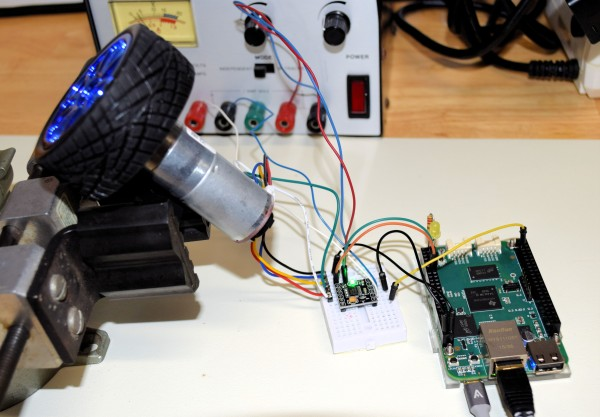
\includegraphics[width=\textwidth]{photos/intro_view}
\end{figure}

\bigskip
{\centering\bfseries\Large
Gregory Raven
\par}


\bigskip
{\centering\bfseries\LARGE
December 28, 2016
\par}
%\newpage





%\setcounter{page}{1}

%\author{Gregory Raven}
%\title{Using the Beaglebone Black Programmable Real-Time Unit with the RemoteProc and Remote Messaging Framework to Capture and Play Data from an ADC}
%\date{October 2016}

%
\frontmatter
Beaglebone Green PRU PID Motor Speed Control Project

Copyright 2016 by Gregory Raven
%\maketitle
\tableofcontents
\listoftables
\listoffigures
%\maketitle

\mainmatter
%    Documentation for PRU ADC Project
%    Copyright (C) 2016  Gregory Raven
%
%    This program is free software: you can redistribute it and/or modify
%    it under the terms of the GNU General Public License as published by
%    the Free Software Foundation, either version 3 of the License, or
%    (at your option) any later version.
%
%    This program is distributed in the hope that it will be useful,
%    but WITHOUT ANY WARRANTY; without even the implied warranty of
%    MERCHANTABILITY or FITNESS FOR A PARTICULAR PURPOSE.  See the
%    GNU General Public License for more details.
%
%    You should have received a copy of the GNU General Public License
%    along with this program.  If not, see <http://www.gnu.org/licenses/>.

\chapter{Introduction}

This is the documentation for an embedded GNU/Linux project utilizing the RemoteProc and RPMsg framework in the Beaglebone Green (BBG) development board.  The project repository is located here:

\url{https://github.com/Greg-R/pru-pid-motor}

The inspiration for this project came from an example project published by Texas Instruments.  The Texas Instruments project is based on "Code Composer Studio".  This
requires a relatively complex cross-compiler installation:

\url{http://processors.wiki.ti.com/index.php/PRU_Training:_PRU_PID_Motor_Demo}

There is also a PDF file which describes the project in detail:

\url{http://www.ti.com/lit/ug/tidubj6/tidubj6.pdf}

Recent developments in the Texas Instruments PRU support include the RemoteProc and Remote Messaging frameworks, as well as an extensively documented C compiler and much additional supporting documentation.  This project utilizes these frameworks and is entirely dependent upon C code in both the PRU and GNU/Linux user space.  For further information, refer to the detailed examples provided by TI in the ``PRU Support Package'':

\url{https://git.ti.com/pru-software-support-package}

A listing of additional resources is found in the Resources chapter.

The motor recommended by TI was purchased and tested.  However, a better motor with an integrated encoder was found on eBay and is recommended.  A chapter is included with describes this motor-encoder and how to obtain one.

%\begin{figure}[H]
%	\centering
%	\includegraphics[width=0.8\textwidth]{diagrams/data_flow_intro}
%	\centering\bfseries
%	\caption{Flow of Data Through the System}
%\end{figure}

\section{Project Goals}

This project demonstrates an electronic speed control for a DC motor which is implemented with the PRUs included with the Beaglebone Green.  Beyond its usefulness as a demonstration project, it could be used in a robotics project such as a ``mobile robot''.


\section{Limitations}

The BeagleBone's Sitara ``System On Chip'' is quite powerful, and this power is probably masking several inefficiencies in the project's design.  All of the testing and debugging was done with a bare-bones Debian distribution with no other significant processes running.

The speaker audio does not have noticeable distortion or glitches when listening with the speaker.  The audio was not examined with a spectrum or distortion analyzer.  It may not be the best quality audio.

The audio sample rate was limited to 8 kHz, which is the lowest rate accepted by ALSA.  A follow-up investigation will see if the sample rate can be increased.  It is not known what aspect of the system will begin to break down as the sample rate is increased.

The sample rate had to be ``tuned'' to prevent ``buffer underruns'' reported by the ALSA system.  An approach to make the real-time data stream robust is not known by the author and needs further investigation.

All of the development was done as root user via ssh on the BeagleBone Green.  This is generally not a good practice, however, considering this as an embedded and experimental project it was not considered to be a serious drawback.



\chapter{System Diagrams}

\begin{figure}[H]
	\centering
	
\includegraphics[width=0.8\textwidth]{diagrams/soc_system}
	\centering\bfseries
	\caption{PRU PID System on BeagleBone Green AM335X ``System On Chip''}
\end{figure}

The above diagram shows the data pathways used in the project.

\section{Programmable Real-time Units (PRU)}

The system uses both PRUs available on the Beaglebone Green:

\begin{enumerate}
\item 

PRU0 implements the PID controller.  The C code in file PRU\_PID\_0.c contains
the math required for the PID controller.  The controlled quantity is the DC motor RPM which is obtained from the Quadrature Encoder.

PRU0 gets performs calculations based on data retrieved (and written to) PRU shared memory.
\item 
PRU1 acts as the master communicator for the system.  PRU1 instantiates two "character devices" via the RemoteProc Messaging framework.  These character devices are used for two-way communication between the PRUs and Linux user-space.  In addition to the supervisory control function, the PWM module on PRU1 is used to drive the DC motor driver IC.

The Quadrature encoder used is not part of the PRU-ICSS.  However, the PRUs have access to the encoders which are part of the AM335X "System On Chip" (SOC).  Access to this encoder is enabled in PRU1 code.
\end{enumerate}

It is worth noting that the PRUs each have a copy of the same ``PWMSS'' (Pulse-Width Modulation Subsystem) as the ones located in the AM335X SOC.  However, only a single pin is connected from the PRU-ICSS to the outside world.  Since this single pin is used for PWM, the decoder-counter function must be done outside the PRU-ICSS thus one of the SOC's eQEP decoder-counters is used and is accessed by PRU1 via the Interface/OCP Master port.

The PWMSS sub-system is surprisingly complex.  A detailed description of the features of this sub-system is available in the AM335x Technical Reference Manual:

\url{http://www.ti.com/lit/ug/spruh73o/spruh73o.pdf}

\section{PRU Shared Memory}

The firmwares running on the two PRUs use a C structure which is placed into "shared memory".  The shared memory is a feature built into the PRU-ICSS architecture.  The shared memory is allocated by an entry in the "linker command file" which is included in the Github repository.

The structure in shared memory allows the two PRUs to synchronize the PID control parameters.  PRU1 receives the parameters via user-space via the character devices and then writes them to shared memory.  This makes the parameters available to PRU0, which is then able to perform PID control loop calculations.  In turn, PRU0 calculates the PWM duty cycle, and this is written to shared memory.  PRU1 then applies this to the PWM output.

PRU1 is responsible for reading the Quadrature Encoder, which is accessed via the OCP bus master.  PRU1 writes this data to shared memory, which enables PRU0 to access this information for PID loop calculations.

A mystery is how the PRUs are able to share memory without locking.  It is possible for the PRUs to simultaneously read and write to the same memory location without introducing errors?

\section{GNU/Linux Operating System on Host ARM Processor}

The command uname -a on the BBG used to develop this project reports this:

\begin{verbatim}
Linux BBG2 4.4.30-ti-r64 #1 SMP Fri Nov 4 21:23:33 UTC 2016 armv7l GNU/Linux
\end{verbatim}

The latest IOT image has a newer kernel.  It is not a major update as of December 18, 2016.

\section{User-space C Program ``prumsg''}

A program runs in GNU/Linux user-space and is used to send commands to PRU1 via character devices instantiated by the RemoteProc messaging framework.  The program can also query PRU1 and return the current state of control variables for the PID as well as the setpoint and RPM reading from the quadrature encoder.

\section{Motor System Diagram}

\begin{figure}[H]
	\centering
	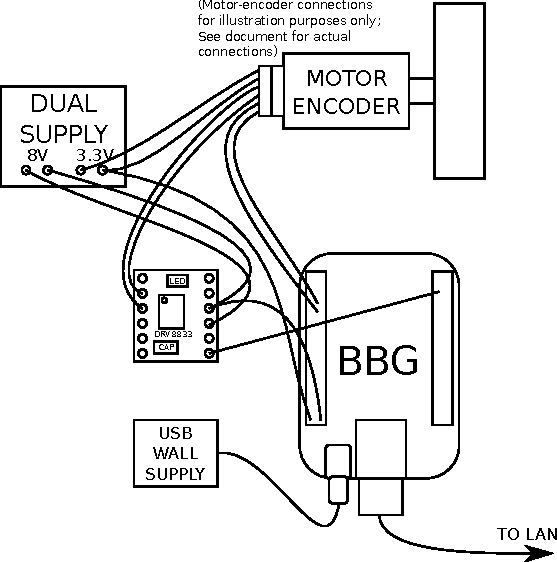
\includegraphics[width=1.0\textwidth]{diagrams/motor_system}
	\centering\bfseries
	\caption{Overall Motor System}
\end{figure}






%    Documentation for PRU ADC Project
%    Copyright (C) 2016  Gregory Raven
%
%    This program is free software: you can redistribute it and/or modify
%    it under the terms of the GNU General Public License as published by
%    the Free Software Foundation, either version 3 of the License, or
%    (at your option) any later version.
%
%    This program is distributed in the hope that it will be useful,
%    but WITHOUT ANY WARRANTY; without even the implied warranty of
%    MERCHANTABILITY or FITNESS FOR A PARTICULAR PURPOSE.  See the
%    GNU General Public License for more details.
%
%    You should have received a copy of the GNU General Public License
%    along with this program.  If not, see <http://www.gnu.org/licenses/>.

\chapter{PRU Firmware and User-space Program}

The ``PRU Firmware'' are two binary files which are placed in the directory /lib/firmware.
These files must have specific names as follows:

\begin{itemize}
	\item am335x-pru0-fw
	\item am335x-pru1-fw
\end{itemize}

The Makefile includes cp commands to copy the firmwares to the /lib/firmware directory.

\section{Implementing the SPI Bus Firmware in C (pru0adc.c)}

The SPI bus C program roughly follows the PRU assembly code written by Derek Molloy.  The C code is compiled to a binary file am335x-pru0-fw. The firmware is loaded into PRU0 automatically by the Remoteproc kernel driver.

The program begins with code sequestered from an example code file in TI's PRU Software
Support Package.  This codes establishes the character device driver via the ``Remote Proc Messenger''
kernel driver.  There are several lines of RPMsg ``set-up'' code which appear at the top of the file.

Here is the path to the file from the root directory of the PRU Software Support Package:

\begin{verbatim}
pru-software-support-package/examples/am335x/PRU_RPMsg_Echo_Interrupt0
\end{verbatim}

There is a sort of ``priming'' process required whereby a user space program writes
to the device driver.  The initializes the character driver, which allows it to write data from
the PRU to the character driver and thus making the data available in user-space.  This is the critical
code which performs this function:

\begin{verbatim}
  //  This section of code blocks until a message is received from ARM.
  while (pru_rpmsg_receive(&transport, &src, &dst, payload, &len) !=
  PRU_RPMSG_SUCCESS) {
  }
\end{verbatim}

This empty while-loop continues until the user-space code writes a message to the character driver.  Upon receipt of a message, the data transport channel is ready to go, and the program breaks out of the while-loop.

After the initialization is complete, the program enters a for-loop.  The SPI bus is implemented inside this for-loop.  This is done by ``bit-twiddling'' of register \_\_R30, which is 32 bits in length.  The individual bits in \_\_R30, in turn determine the ``high'' or ``low'' state at the GPIO, and thus the header pins.  The GPIO multiplexing is set via the ``Universal IO'', which is described in a later chapter.

The code utilizes timing delays and sequential setting and unsetting of bit values of \_\_R30.  This is done per the requirements shown in the MCP3008 ADC data sheet. Each pass through the for-loop configures the ADC, and then captures a single 10-bit sample from the ADC.

The top of the for-loop is blocked by a while ``polling'' loop.  The operand of the while-loop is the value of a PRU shared memory location.  The PRU1 timing clock code writes to this location at precisely timed intervals.  When the while loop detects that three of the bits change from 0s to 1s, the while loop is broken and the SPI bus data acquisition sequence begins.  This action is what determines the 8 kHz data sampling rate.

The samples are accumulated in a buffer (int16\_t payload[256]).  When the buffer is filled, the data is written to the character device via a function provided by the RPMsg kernel driver.  Here is the code:

\begin{verbatim}
    //  Send frames of 245 samples.
    //  The entire buffer size of 512 can't be used for
    //  data.  Some space is required by the "header".
    //  The data is offset by 512 and then multiplied
    //  to make appropriately scaled 16 bit signed integers.
    payload[dataCounter] = 50 * ((int16_t)data - 512);
    dataCounter = dataCounter + 1;
    
    if (dataCounter == 245) {
    pru_rpmsg_send(&transport, dst, src, payload, 490);
    dataCounter = 0;
    }
\end{verbatim}

The dataCounter variable is incremented at the end of each pass through the for loop.  When the dataCounter hits 245, the pru\_rpmsg\_send command is used to write data to the character device. The dataCounter variable is reassigned to zero and the process repeats.

The maximum buffer size which can be handled by RPMsg is 512 bytes (or 256 16 bit integers).  However, not all of the buffer can be used as there is a ``header'' included which takes a few bytes.  The number of samples transmitted, 245, was determined empirically.  Some study of the kernel drivers needs to be accomplished to better understand this limitation.

Timings are critical, and this was accomplished by using the compiler intrinsic \_\_delay\_cycles.  Each delay is an absolute value of 5 nanoseconds.  This scheme has sufficient timing precision to implement the SPI bus in real time.  

\section{Implementing the Timing Clock Firmware in C (pru1adc.c)}

The ``Timing Clock'' sets the data sample rate.  The code is compiled into firmware am335x-pru1-fw, and this binary file is loaded into PRU1 by the Remoteproc kernel driver.

The output of the Timing Clock is a single pulse at a rate of 8 kHz.  This pulse is written to a PRU shared memory location.  This means that the SPI program in PRU0 can access this memory address and read its state.  A while loop in PRU0 polls this address and exits from the loop when the pulse goes high.  This polling action is done at the top of the for loop which captures a data sample from the ADC.  Thus the data capturing sequence in PRU0 is gated at the Timing Clock pulse rate.

The Timing Clock does not begin emitting pulses as soon as the firmware is loaded and started.  There is a character device created in the initialization section of the C code.  The character device is created, and then a while loop begins monitoring for a specific incoming message, which in this case is the letter ``g'' (go);  When the go message is successfully received, the while loop is exited and the Timing Clock pulse code begins emitting pulses to PRU shared memory.  Here is the code snippet which does this:

\begin{verbatim}
 //  The following code looks for a specific incoming message via RPMsg.
 //  This code blocks until the message is successfully received.
 //  If the correct message is received, the clock is allowed to begin.
  while (1) {
    /* Check bit 30 of register R31 to see if the ARM has kicked us */
    if (__R31 & HOST_INT) {
      /* Clear the event status */
      CT_INTC.SICR_bit.STS_CLR_IDX = FROM_ARM_HOST;
      /* Receive all available messages, multiple messages can be sent per kick
       */
      if (pru_rpmsg_receive(&transport, &src, &dst, payload, &len) ==
          PRU_RPMSG_SUCCESS) {
        if (payload[0] == 'g')
          break;
      }
    }
  }
\end{verbatim}

After the ``go'' code is successfully received, the pulse timing code begins.

The pulse timing code is contained in an infinite while-loop.  A pointer variable is declared which is the address of the PRU shared memory location.  This pointer is ``dereferenced'' and the value 7 (binary LSB value 111) to pulse ``high'', a delay command fires which defines the pulse width, and then the deferenced pointer is reassigned to zero.

The manipulation of \_\_R30 is done so that the pulse is also present at the header pin P9.30.  This allows monitoring via the Analog Discovery 2 logic analyzer.

\begin{verbatim}
  //  The sample clock is located at shared memory address 0x00010000.
  //  Need a pointer for this address.  This is found in the linker file.
  //  The address 0x0001_000 is PRU_SHAREDMEM.
  uint32_t *clockPointer = (uint32_t *)0x00010000;
  *clockPointer = 0; //  Clear this memory location.

  while (1) {
    __R30 = __R30 | (1 << 11);  // P9.30
    *clockPointer = 7;
    __delay_cycles(1000); 
    *clockPointer = 0;
    __R30 = __R30 & (0 << 11);
    //  The following delay will set the clock rate.
    //  This delay was originally 24000 cycles; it was reduced due to ALSA underruns.
    __delay_cycles(23980); 
  }
\end{verbatim}

The final line of the delay loop using the compiler intrinsic \_\_delay\_cycles(23980) sets the pulse rate.  Each delay cycle is 5 nanoseconds, and the pulse rate can be computed as follows:

\[ \frac{\text{1}}{1000*5ns + 24000*5ns}  = \text{8000 Hz} \]

Note that a few cycles are also required to implement the while-loop and to change the state of \_\_R30.  With the total value of 25000 delays, ALSA emitted ``buffer underrun'' warnings.  The delay value was empirically reduced until the underrun notices were no longer emitted.


%    Documentation for PRU ADC Project
%    Copyright (C) 2016  Gregory Raven
%
%    This program is free software: you can redistribute it and/or modify
%    it under the terms of the GNU General Public License as published by
%    the Free Software Foundation, either version 3 of the License, or
%    (at your option) any later version.
%
%    This program is distributed in the hope that it will be useful,
%    but WITHOUT ANY WARRANTY; without even the implied warranty of
%    MERCHANTABILITY or FITNESS FOR A PARTICULAR PURPOSE.  See the
%    GNU General Public License for more details.
%
%    You should have received a copy of the GNU General Public License
%    along with this program.  If not, see <http://www.gnu.org/licenses/>.

\chapter{RemoteProc and RPMsg Framework}

\begin{figure}[h]
	\centering
    
\includegraphics[width=0.7\textwidth]{diagrams/soc_system}
	\centering\bfseries
	\caption{PRU<->ARM Character Devices}
\end{figure}

TI has provided example code and kernel drivers for the ``RemoteProc and RemoteProc Messaging Framework''.  A detailed explanation of this framework is available here:

\url{http://processors.wiki.ti.com/index.php/PRU-ICSS_Remoteproc_and_RPMsg}

This framework provides a means of controlling and communicating with the PRUs from user-space, and this project is totally dependent on these functions.

The Remoteproc framework automatically does the job of loading the PRU firmwares from user-space into the PRUs.  Via a sysfs entry, the PRUs can be started and halted from the command line.  These functions are described in the chapter "Shell Scripts".

The examples provided in the PRU Software Support Package show how to use provided functions to send and receive data from PRU to ARM or ARM to PRU.  This is done via character devices which appear in the usual /dev directory.  The standard POSIX functions read/write/open/close work with these character devices.  This allows for typical systems programming technique to become applicable when working with the PRUs.

This project requires the use of one character device for each PRU.  The character driver for PRU0 is the ``data stream'' for PCM data read from the ADC via the SPI bus.  The character device for PRU1 is used to activate the PRU1 Timing Clock as the last action after all systems are initialized.  A simple signal is transmitted from user-space to PRU1, and this begins the flow of data through the system.

This project did not require modifications to the loadable kernel modules in the Remoteproc framework.  The modules provided with the support package were used as-is.

\section{The Remoteproc and RPMsg Kernel Modules}

``Loadable Kernel Modules'' (LKMs) must be active for this project to function.
At the shell command line, execute this command:

\begin{verbatim}
lsmod
\end{verbatim}

This will list the LKMs currently loaded.  The modules associated with Remoteproc are:

\begin{itemize}
\item pruss
\item pru\_rproc
\item pruss\_intc
\end{itemize}

There are two modules associated with RPMsg, and these will appear in the list only after the firmwares are loaded into the PRUs:

\begin{verbatim}
virtio_rpmsg_bus
rpmsg_pru
\end{verbatim}

The Remoteproc kernel modules may not be loaded at boot (depending on boot configuration).  However, they can be loaded (or unloaded) anytime after boot with the following commands:

\begin{verbatim}
modprobe pru_rproc
rmmod pru_rproc
\end{verbatim}

``modprobe'' is the load command; rmmod is the remove command.

Perhaps a better method of controlling the Remoteproc framework is via the sys virtual file system.  A set of shell scripts is included in the repository which includes these commands in the ``prumodout'' and ``prumodin'' scripts.

\section{Files Associated with RemoteProc in the Compilation Process}

There are some interesting files in the root directory of the github repository for this project:

\begin{itemize}
\item resource\_table\_0.h
\item resource\_table\_1.h
\item AM335x\_PRU.cmd
\end{itemize}

These files were copied verbatim from the PRU Support Package.

Jason Reeder of Texas Instruments has provided an explanation of the files required to compile firmwares for the PRUs:

\begin{quotation}
There are four files needed in order to build a C project for the PRU using TI's C compiler. Each of the examples and labs in the pru-software-support-package include these files:
\begin{enumerate}

\item  yourProgramFile.c

This is your C program that you are writing for the PRU.

\item   AM335x\_PRU.cmd

This is a command linker file. This is the way that we describe the physical memory map, the constant table entries, and the placement of our code and data sections (into the physical memory described at the top of the file) to the PRU linker. There are some neat things that can be done as far as placing code and data in exact memory locations using this file, but for the majority of projects, this file can remain unchanged.

\item   resource\_table\_*.h

This file will create a header in the elf binary (generated .out file) that is needed by the RemoteProc Linux driver while loading the code into the PRUs. For the examples in the pru-software-support-package, there are two types of resources that the PRU can request using the resource\_table\_*.h file:

interrupts - letting RemoteProc configure the PRU INTC interrupts saves code space on the PRUs.

vrings - requesting vrings in the resource\_table file is necessary if rpmsg communication is desired (since the ARM/Linux needs to create the vrings in DDR and then notify the PRU where the vrings were placed)
even if no resources are needed, the RemoteProc Linux driver expects the header to exist. Because of this, many examples in the package contain an empty resource\_table header file (resource\_table\_empty.h)

\item   Makefile

Makefile to build your PRU C program either on the target, on your Linux machine, or even on a Windows machine. The comment at the top of the Makefile tries to explain the environment variable needed for a successful build and how to set it on each of the three supported build development environments.

\end{enumerate}
\end{quotation}








%    Documentation for PRU ADC Project
%    Copyright (C) 2016  Gregory Raven
%
%    This program is free software: you can redistribute it and/or modify
%    it under the terms of the GNU General Public License as published by
%    the Free Software Foundation, either version 3 of the License, or
%    (at your option) any later version.
%
%    This program is distributed in the hope that it will be useful,
%    but WITHOUT ANY WARRANTY; without even the implied warranty of
%    MERCHANTABILITY or FITNESS FOR A PARTICULAR PURPOSE.  See the
%    GNU General Public License for more details.
%
%    You should have received a copy of the GNU General Public License
%    along with this program.  If not, see <http://www.gnu.org/licenses/>.

\chapter{Device Tree Requirements}

This project requires a custom ``Device Tree Include''.  This is a device tree fragment which is inserted into the top device tree file.  The dtsi directory located in the software directory contains the file and and a README file which explain how to edit the device tree source file.

The same file, which in this case is ``am335x-bonegreen.dts'', must be modified in order to active the RemoteProc framework kernel drivers.  It is recommended to add the include statement at the same time the RemoteProc is activated.  This step is included in the RemoteProc and PRU Compiler step-by-step process in Chapter 9.


There is one PRU GPIO output enabled on header P9 and this is used to monitor Quadrature Decoder under/overflow.  This configuration is done in the same file ``pru\_gpio\_config'' which is sourced by .bashrc as will be discussed in Chapter 8.

The Universal IO project is located at this Github repository:

\url{https://github.com/cdsteinkuehler/beaglebone-universal-io}

Universal IO is included with the most recent Debian-based IOT images.






%    Documentation for PRU ADC Project
%    Copyright (C) 2016  Gregory Raven
%
%    This program is free software: you can redistribute it and/or modify
%    it under the terms of the GNU General Public License as published by
%    the Free Software Foundation, either version 3 of the License, or
%    (at your option) any later version.
%
%    This program is distributed in the hope that it will be useful,
%    but WITHOUT ANY WARRANTY; without even the implied warranty of
%    MERCHANTABILITY or FITNESS FOR A PARTICULAR PURPOSE.  See the
%    GNU General Public License for more details.
%
%    You should have received a copy of the GNU General Public License
%    along with this program.  If not, see <http://www.gnu.org/licenses/>.

\chapter{Shell Scripts}

\section{RemoteProc ``Bind'' and ``Unbind'' Commands}

There are two very important shell scripts located in the shell\_scripts of the git repository.

These scripts are very simple and each contain only a single command.

The commands are described in the notes file from this github repository:

\url{https://github.com/ZeekHuge/BeagleScope}

And specifically, this is the path to the notes file:

\url{https://github.com/ZeekHuge/BeagleScope/blob/port_to_4.4.12-ti-r31%2B/docs/current_remoteproc_drivers.notes} 
	
	The commands are seen in section 2:
	
	\begin{verbatim}
	echo "4a334000.pru0" > /sys/bus/platform/drivers/pru-rproc/unbind
	echo "4a334000.pru0" > /sys/bus/platform/drivers/pru-rproc/bind
	echo "4a338000.pru1"  > /sys/bus/platform/drivers/pru-rproc/unbind
	echo "4a338000.pru1" > /sys/bus/platform/drivers/pru-rproc/bin
	\end{verbatim}
	
	The above shell commands show how the PRUs can ``bind'' and ``unbind'' from the remoteproc driver.  These commands are extremely useful and their placement in shell scripts allows them to be easily run at the command line by entering ``prumodin'' or ''prumodout''.
	
	The shell scripts should be copied to /usr/bin to make them available from any shell.
	
\section{Environment Variables and Universal IO Configuration Script}

The make process which compiles the PRU firmwares requires an environment variable to be set:

\begin{verbatim}
export PRU_CGT=/usr/share/ti/cgt-pru
\end{verbatim}

This is best done by writing this export statement plus other configurations to a file.
This file is sourced from the .bashrc file upon entering the home directory bash shell.

Other methods of setting the environment variables were tried. Using .bashrc was found to be the most practical.

When using the ``sudo'' command to gain temporary root access, it is necessary to use the -E option in order to preserve the environment variables.  For example:

\begin{verbatim}
sudo -E make
\end{verbatim}

will preserve the \$PRU\_CGT environment variable and will allow the successful compilation of the PRU firmwares.

The file ``pru\_gpio\_config'' is included in the shell\_scripts directory.  Source the file by adding this line to the end of the .bashrc file located in the user home directory:

\begin{verbatim}
source /home/debian/pru-pid-motor/software/shell_scripts/pru_gpio_config
\end{verbatim}

The path shown above assumes the project was cloned to the user's home directory (debian by default in the latest distribution).

%    Documentation for PRU ADC Project
%    Copyright (C) 2016  Gregory Raven
%
%    This program is free software: you can redistribute it and/or modify
%    it under the terms of the GNU General Public License as published by
%    the Free Software Foundation, either version 3 of the License, or
%    (at your option) any later version.
%
%    This program is distributed in the hope that it will be useful,
%    but WITHOUT ANY WARRANTY; without even the implied warranty of
%    MERCHANTABILITY or FITNESS FOR A PARTICULAR PURPOSE.  See the
%    GNU General Public License for more details.
%
%    You should have received a copy of the GNU General Public License
%    along with this program.  If not, see <http://www.gnu.org/licenses/>.

\chapter{Setting up the Remoteproc Framework and PRU Compiler on the Beaglebone Green}

The following describes the simplest possible set-up.  Everything was done via the command line, and the vim editor was used extensively to develop the C code and shell scripts.

SSH was used to remotely access the BBG from a 64 bit desktop computer running Ubuntu 14.04.

For reference, here is the link to the TI PRU support package:

\url{https://git.ti.com/pru-software-support-package}

The above package can be cloned to the BBG.  There is a good set of examples and labs included.  The labs are documented here:

\url{http://processors.wiki.ti.com/index.php/PRU_Training:_Hands-on_Labs}

Note that the files appropriate for the BBG are in the folders with name am335x.

The Makefiles in the labs and examples were designed to work with a particular set-up which can be easily implemented on the BBG.

The following is a list of recommended steps to prepare a BBG for compiling PRU C files.
This process assumes a relatively new SD card image which is loaded with the PRU compiler (clpru) and libraries.  Another assumption is that the Remoteproc and RPMsg kernel drivers are included and that they are loaded during the start-up process.  This is true for some, but not all, recently published images as of November, 2016.

\section{Activate Remoteproc PRU and Kernel Modules}

The newest Beaglebone Debian distributions do not have the Remoteproc framework activated by default!

The following process activates the framework which includes several loadable kernel modules.  This is a prerequisite for the remainder of the setup process.

This process was tested using this image:

bone-debian-8.6-iot-armhf-2016-10-30-4gb.img

The ``IOT'' (Internet Of Things) image includes the set of tools required to install and compile the required software.
The image was found at this web site:

\url{http://elinux.org/Beagleboard:BeagleBoneBlack_Debian#microSD.2FStandalone:_.28iot.29_.28BeagleBone.2FBeagleBone_Black.2FBeagleBone_Green.29}

The IOT distribution includes very useful scripts in the following directory:

/opt/scripts/tools

The script grow\_partition.sh will expand the file system on the microsd card to its full capacity.  Running this script is highly recommended before proceeding with this process!

\section{Activate Remoteproc: Step-by-step Process}

\begin{enumerate}
\item  Write Beaglebone image to micro-sd and expand partition as required.
\item  Insert micro-sd into BBG slot, press boot and power buttons and release.  Non-flasher images may not require the boot button to be pressed, and the board will boot and run from the SD card.
\item  ssh debian@192.168.1.7 (or whatever the IP is set to).  If you are using a router with a GUI control application, it may have a display which indicates the board is connected and which IP address has been assigned to it.
\item  Execute
\begin{verbatim}
sudo apt-get update
\end{verbatim}
\item  Execute
\begin{verbatim}
uname -r
\end{verbatim} 
to verify kernel version.  Please note that the Remoteproc framework is still evolving and it is recommended to verify that the kernel used will work with the PRU support package examples.

The rest of the set-up will be completed using root access.
Execute
\begin{verbatim}
sudo su
\end{verbatim}
and authenticate as required to switch to root user.
\item Clone this repository to a convenient directory:

\begin{verbatim}
git clone https://github.com/RobertCNelson/dtb-rebuilder
\end{verbatim}

\item Execute:
\begin{verbatim}
cd dtb-rebuilder/ 
cd src/arm
\end{verbatim}
\item Find and edit the top of the device tree dts file.
For BBG, this is:
\begin{verbatim}
am335x-bonegreen.dts
\end{verbatim}
Uncomment this single line in the file:
\begin{verbatim}
/*   #include "am33xx-pruss-rproc.dtsi"  */
\end{verbatim}

The line should now look like this:
\begin{verbatim}
#include "am33xx-pruss-rproc.dtsi"
\end{verbatim}

A new include statement must be added to the same file for configuration of the Quadrature Decoder and the PRU PWM.  This file must be copied from the repository:

\begin{verbatim}
pru-pid-motor/software/dtsi/am335x-boneblack-prupid.dtsi
\end{verbatim}

into the arm directory in the dtb-rebuilder.

Add this line to the end of the am335x-bonegreen.dts file:

\begin{verbatim}
#include "am335x-boneblack-prupid.dtsi"
\end{verbatim}
 
Save and exit.
\item
Execute:
\begin{verbatim}
cd /etc/modprobe.d
\end{verbatim}
Create a new file named:
\begin{verbatim}
pruss-blacklist.conf
\end{verbatim} 

Add this single line to the file:
\begin{verbatim}
blacklist uio_pruss
\end{verbatim}
Save and exit.
\item
cd back to the dtb-rebuilder directory.  Execute these commands:
\begin{verbatim}
make 
make install 
reboot
\end{verbatim} 
\end{enumerate}
To verify that the above process was successful:

\begin{verbatim}
cd /sys/bus/platform/devices
ls
\end{verbatim}

Now look for the following in the output from the ls command:
\begin{verbatim}
4a300000.pruss
4a320000.intc
4a334000.pru0
4a338000.pru1
\end{verbatim}

The appearance of the above entries indicates that the Remoteproc PRU activation process was successful.

\section{PRU Compiler Setup Process}
\begin{enumerate}
\item  Execute these commands:
  \begin{verbatim}
cd /
\end{verbatim} and then 
\begin{verbatim}
find . -name cgt-pru
\end{verbatim}

The path may be something like 
\begin{verbatim}
/usr/share/ti/cgt-pru
\end{verbatim}  

This is the location of the PRU library and includes.
However, the clpru compiler binary is not located in this directory.  Run this command:
\begin{verbatim}
which clpru
\end{verbatim}
and the result will be something like:
\begin{verbatim}
/usr/bin/clpru
\end{verbatim}
This is the path to the compiler binary.

The PRU C compiler needs to find the include and lib directories.  Execute the following:

\begin{verbatim}
cd /
find . -name cgt-pru
\end{verbatim}

This should find the following or similar path:

\begin{verbatim}
/usr/share/ti/cgt-pru
\end{verbatim}

The above is the path to the C Compiler includes and lib directories.  The Makefiles in the PRU Support Package look for the compiler binary at this path, so the following changes must be made.

Execute the following commands (as root):
\begin{verbatim}
cd /usr/share/ti/cgt-pru
mkdir bin
cd bin
ln -s /usr/bin/clpru clpru
\end{verbatim}
So now the Makefiles will find the compiler executable in the correct location via the link.
\item  Now install the PRU Support Package:

\begin{verbatim}
cd /home/debian
git clone git://git.ti.com/pru-software-support-package/pru-software-support-package.git
\end{verbatim}

This will clone a copy of the latest pru support package.
\item  cd into lab\_5 in the package and execute the make command:
\begin{verbatim}
cd pru-software-support-package/labs/lab_5/solution/PRU_Halt
make
\end{verbatim}
This will fail, as the Makefile is looking for environment variable \$PRU\_CGT.  Execute:

\begin{verbatim}
export PRU_CGT=/usr/share/ti/cgt-pru
\end{verbatim}

Now execute the make command again.  It should succeed.  A new directory ``gen'' should appear.  Add the above export command to the start-up commands (.profile or .bashrc).
\item  Execute the following:
\begin{verbatim}
cd gen
cp PRU_Halt.out am335x-pru0-fw
cp am335x-pru0-fw /lib/firmware
\end{verbatim}
This renames the executable binary and copies it to the directory at which Remoteproc expects to find PRU firmwares.
\item  Now cd into the PRU\_RPMsg\_Echo\_Interrupt1 directory in the same lab\_5.
Edit main.c as follows:
\begin{verbatim}
//#define CHAN_NAME					"rpmsg-client-sample"
#define CHAN_NAME					"rpmsg-pru"
\end{verbatim}
The ``CHAN\_NAME'' define is now set to ``rpmsg-pru''.
\item  Now execute almost the same as \#9, except this time the firmware for PRU1 is compiled a copied:
\begin{verbatim}
make
cd gen
cp PRU_RPMsg_Echo_Interrupt1.out am335x-pru1-fw
cp am335x-pru1-fw /lib/firmware
\end{verbatim}
The compilation of both PRU firmwares are complete and they are copied to /lib/firmware.
\item  reboot
\item  Execute:

\begin{verbatim}
lsmod
\end{verbatim}

These kernel modules should be present in the output:

\begin{verbatim}
pru_rproc              15431  0 
pruss_intc              8603  1 pru_rproc
pruss                  12026  1 pru_rproc
\end{verbatim}
Now execute:
\begin{verbatim}
rmmod pru_rproc
modprobe pru_rproc
\end{verbatim}

The rmmod command removes the remoteproc module pru\_rproc.
The modprobe command re-inserts the same module.
\item  
\begin{verbatim}
cd /dev
ls
\end{verbatim} 

Look for rpmsg\_pru31 character device file.  It will be there!
\end{enumerate}

\section{Additional Configuration Required to Compile the PRU Remoteproc Project}

Some components of the PRU Support Package need to be added to the PRU C compiler directories.  The Makefile expects to find these components in these directories.


Execute these commands:

\begin{verbatim}
cd pru-software-support-package/
cp -r include $PRU_CGT/includeSupportPackage
cp lib/rpmsg_lib.lib $PRU_CGT/lib
\end{verbatim}

This should complete the configuration required to run the command successfully.




\chapter{Using the Analog Discovery 2}



This table shows the Discovery 2 to PRU-ADC cape connections.


	\begin{longtable}{cllc}
		\caption{Analog Discovery 2 Wiring}\\
		\toprule
Logic Wire Number & Color & SPI & BBG Header \\\midrule
	1	& Green & Chip Select & P9.27 \\ 
	2	& Purple & Clock & P9.30 \\ 
	3	& Brown & MISO & P9.28 \\ 
	4	& Pink &  MOSI & P9.29 \\ 
	5	& Green & PRU1 Clock & P8.30 \\
	\bottomrule
	\end{longtable}
	
	The repository includes a set-up file for the Analog Discovery 2 in the ``discovery2'' directory.  The Logic Analyzer will appear as in the image below.
	
	\begin{figure}[H]
		\centering
		\includegraphics[width=0.8\textwidth]{photos/discovery2_logic}
		\centering\bfseries
		\caption{Analog Discovery 2 Logic Analyzer Display}
	\end{figure}
	
	The Analog Discovery also includes an audio waveform generator, and it will appear in the GUI as shown in this image:
	
		\begin{figure}[H]
			\centering
			\includegraphics[width=0.8\textwidth]{photos/discovery2_waveform}
			\centering\bfseries
			\caption{Analog Discovery 2 Waveform Generator Display}
		\end{figure}
		
		



	
	

\chapter{Running the Project}

It is assumed the numerous steps described in prior chapters have been completed to enable the RemoteProc framework drivers and configure the BBG for compiling PRU C code.  The Device Tree must have been successfully edited and re-compiled and installed, and the shell scripts prumodin and prumodout have been copied to /usr/bin.

In order to run the project and successfully control the motor, follow these steps:

\begin{itemize}
	\item run ``make'' in the software repository directory.  Some warnings or errors may be ignored.  Check that the C code files prumsg.c, PRU\_PID\_0.c and PRU\_IO\_1.c compile and firmware files am335x-pru0-fw and am335x-pru1-fw are copied to /lib/firmware.  The user-space binary prumsg should be copied to /usr/bin.
	
	\item Run command 
	
	\begin{verbatim}
	prumodin
	\end{verbatim} 
	
	at the command line.  This command should start firmware execution in the PRUs.
	If all goes well, the motor should begin turning with a default setpoint value of 3000.
	
	\item  Finally, the user-space program can be used.
	
	\begin{verbatim}
	sudo ./prumsg s 4000
	\end{verbatim}
	
	The above command changes the setpoint to 4000 rpm.  The motor speed should increase.
\end{itemize}

The PRU firmwares will continue to run.  To stop them, issue the commands

\begin{verbatim}
sudo prumodout
sudo rmmod pru_rproc
sudo rmmod pruss
\end{verbatim}

at the command line, and the PRUs will be halted.  The motor will stop.

\section{User-space Program prumsg Command Listing}

The user-space executable file prumsg is capable of several control and monitoring functions.  These commands are issued from a shell and a complete listing of the possible commands is listed below.

\begin{longtable}{ll}
\caption{Commands of User-space Program prumsg}\\
\toprule
Example command & Command function \\\midrule
prumsg 30 s 5000 & Set setpoint (RPM) \\ 
prumsg 30 p 300 & Set Kp, proportional feedback coefficient \\ 
prumsg 30 i 300 & Set Ki, integral feedback coefficient \\ 
prumsg 30 d 300 & Set Kd, derivative feedback coefficient \\ 
prumsg 30 o 3000 & Set output PWM duty cycle (see note below) \\ 
prumsg 30 rs & Readback setpoint (RPM) \\ 
prumsg 30 rp & Readback Kp \\ 
prumsg 30 ri & Readback Ki \\ 
prumsg 30 rd & Readback Kd \\ 
prumsg 30 re & Readback encoder RPM \\
prumsg 30 ro & Readback output PWM
\end{longtable}

Notes on the above:
\begin{enumerate}
\item If not operating as root, ``sudo'' will be required.
 
\item ``30'' in the table above refers to the character device /dev/rpmsg\_pru30.  ``31'' can also be used, as this character device is also established between PRU1 and user-space.
 
\item The example for setting the PWM (prumsg 30 o 3000) will not have effect with the PID controller running.  However, this command is useful for debugging purposes.  If the PID controller is not running in PRU0, then the command will work and the PWM output will change.  The simplest way to do this is to remove firmware am335x-pru0-fw from directory /lib/firmware.  Reboot and restart the system.  PRU1 will still function in system control mode, but the PID calculations will not be performend by PRU0 and the system will operate in ``open-loop'' mode.  This is excellent for checking the PWM output to the motor driver IC and the motor connections.  The motor should properly respond to changes in the PWM duty cycle by issuing the prumsg 30 s (pwm value) command.
\end{enumerate}

\section{Server and GUI Interface from TI Project}

The TI project includes a very clever PHP web page and server interface.  This was found to be mostly functional, and the server shell script and web page implementation is included in the pru\_pid\_server directory of the Git repository.

The server is easy to run.  Simply copy the contents of the pru\_pid\_server directory to /var/www/html which should already be included in the Beaglebone Green IOT image.

Now, using a browser on the local network, browse to this URL:

\begin{verbatim}
10.0.0.2:8080
\end{verbatim}

In the above example, the BBG is set to a static IP of 10.0.0.2.

This was found to partially function, the graphics successfully updates, however, the capability to update the setpoint and PID parameters did not function.

This project does not support this function.  Since the Beagleboard project is heavily invested in node.js and ``Bonescript'', it would probably make sense to change this function from PHP/html to a node-based web interface and use a web-socket for data exchange and parameter control.  This feature may be added in the future to this project.

%    Documentation for PRU ADC Project
%    Copyright (C) 2016  Gregory Raven
%
%    This program is free software: you can redistribute it and/or modify
%    it under the terms of the GNU General Public License as published by
%    the Free Software Foundation, either version 3 of the License, or
%    (at your option) any later version.
%
%    This program is distributed in the hope that it will be useful,
%    but WITHOUT ANY WARRANTY; without even the implied warranty of
%    MERCHANTABILITY or FITNESS FOR A PARTICULAR PURPOSE.  See the
%    GNU General Public License for more details.
%
%    You should have received a copy of the GNU General Public License
%    along with this program.  If not, see <http://www.gnu.org/licenses/>.

\chapter{Resources}


Github repository for this project:

\url{https://github.com/Greg-R/pru-pid-motor}

The Texas Instruments PRU PID Motor Demonstration project:

\url{http://processors.wiki.ti.com/index.php/PRU_Training:_PRU_PID_Motor_Demo}

There is also a PDF file which describes the project in detail:

\url{http://www.ti.com/lit/ug/tidubj6/tidubj6.pdf}

Texas Instruments PRU Code Generation tools:

\url{http://software-dl.ti.com/codegen/non-esd/downloads/download.htm#PRU}

Beagle Bone Green:

\url{https://www.seeedstudio.com/SeeedStudio-BeagleBone-Green-p-2504.html}

The Remoteproc Framework and Remote Messaging:

\url{http://processors.wiki.ti.com/index.php/PRU-ICSS_Remoteproc_and_RPMsg}


The BeagleScope project:

\url{https://github.com/ZeekHuge/BeagleScope}


\backmatter
% bibliography, glossary and index would go here.

\end{document}
